\documentclass[
    10pt,
    journal,
    compsoc,
    english
]{IEEEtran}
\usepackage[T1]{fontenc}
\usepackage{babel}
\usepackage[nocompress]{cite}
\usepackage{graphicx}
\usepackage{amsmath}
\usepackage{amssymb}
\usepackage{dsfont}
\interdisplaylinepenalty=2500
\usepackage{algpseudocodex}
\usepackage{array}
\usepackage{hyperref}
\usepackage{float}
\usepackage{menukeys}
\usepackage{microtype}

%%%%%%%%%%%%%%%%%%%%%%%%%%%%%%%%%
%% Configuraciones adicionales %%
%%%%%%%%%%%%%%%%%%%%%%%%%%%%%%%%%
\makeatletter

%% Algpseudocodex restyling %%
\renewcommand{\algpx@commentFormat}[1]{%
	\ifbool{algpx@italicComments}{%
		\textsl{\textcolor{\algpx@commentColor}{#1}}%
	}{%
		\textcolor{\algpx@commentColor}{#1}%
	}%
}

%% myalg extra commands %%

%% myalg environment %%
\newenvironment{myalg}{%algorithm
    \begin{minipage}{0.95\columnwidth}
    \newcommand{\Var}[1]{\texttt{##1}}
    \selectlanguage{english}
    \hrule width \textwidth\relax\vskip .75em\relax
    \begin{algorithmic}%
}{%
    \end{algorithmic}
    \vskip .75em\relax\hrule width \textwidth\relax
    \end{minipage}%
}

%% Float new environments %%
\newfloat{algorithm}{tbp}{loa}
\floatname{algorithm}{Algorithm}

\makeatother
\endinput
\graphicspath{{./img/}}
\DeclareGraphicsExtensions{.pdf,.jpeg,.png}
\hypersetup{
    colorlinks=true,
    allcolors=blue!75!black
}

% Title info
\markboth{Statistical Mechanics, 2023}{Statistical Mechanics, 2023}

\title{Montecarlo Simulation of the\\Classical 2D--Ising Model}

\author{Abel~Hernández~(\texttt{201980021}),
        Alessandro~Lavagnino~(\texttt{201907400}),
        Amado~Cabrera~(\texttt{201905757}),
        Mariana~Pérez~(\texttt{201901040}),
        and~Samuel~Tzunux~(\texttt{201908333})}

% Abstract and keywords
\IEEEtitleabstractindextext{%
\begin{abstract}
We present a complete implementation of the Ising model based on the class--object paradigm. The model consists of discrete variables that represent magnetic dipole moments of atomic spin that can be in one of two states ($+1$ or $-1$). The model allows for the identification of phase transitions as a simplified model of reality. With that model we could replicate the evolution of a random state through many Monte Carlo steps, and we could also provide plots that illustrate the behavior of different physical properties around the critical temperature point.
\end{abstract}


\begin{IEEEkeywords}
Ising Model, Simulation, Monte Carlo, Metropolis algorithm, Python.
\end{IEEEkeywords}}

\begin{document}

\maketitle

\IEEEraisesectionheading{%
    \section{Introduction}\label{sec:introduction}%
}
\IEEEPARstart{T}{he} Ising model is a widely recognized model in Statistical Mechanics used to study ferromagnetism, which refers to the phenomenon where materials display alignment of magnetic moments. However, the Ising model has a variety of applications in different fields.

In social science it can serve as a tool for examining collective behaviors associated with opinion formation, such as consensus decision-making \cite{social}. Similar to the influence of neighboring spins in the Ising model, voter models propose a network where people change their opinion by being affected by those in close proximity to them.

Another interesting application of the Ising model is in the field of genetics: the simplified Ising model with only nearest-neighbor interactions between genetic markers can detect susceptibility loci\footnote{Loci, plural of locus, term used to indicate where a specific gene is located on a chromosome \cite{loci}.} for type-1 diabetes not previously found by other methods of analysis \cite{genetics}.

The idea that an image can be represented as a certain configuration of Ising spins allows the model to be used for interpolation of spatial data, for example, when some parts of a satellite photo of a certain area are missing due to cloudiness \cite{spatialint}. On the other hand, a relatively small fraction of spins is enough for a reliable restoration of an entire biometric template \cite{biometric}.


\section{Model Description}
\subsection{Classical Ising Model Description}
The Ising model is a mathematical model of ferromagnetism in Statistical Mechanics. The model consists of discrete variables that represent magnetic dipole moments of atomic ``spin'' that can be in one of two states ($+1$ or $-1$). The spins are arranged in a graph, usually a lattice (where the local structure repeats periodically in all directions), allowing each spin to interact with its neighbors. Neighboring spins that agree have a lower energy than those that disagree; the system tends to the lowest energy but heat disturbs this tendency, thus creating the possibility of different structural phases. The model allows the identification of phase transitions as a simplified model of reality. The two-dimensional square--lattice Ising model is one of the simplest statistical models to show a phase transition \cite{IsingModelEn}.

In summary, the magnetic behavior depends on the temperature, therefore, we can have three cases:
\begin{enumerate}
    \item At high temperature, thermal excitation cause the spins to readily change orientation and there is little organization in the system.
    \item As the temperature decreases, lower-energy states are favored. These are attained when neighboring spins agree, cause small aligned domains to form.
    \item Once this alignment translates to a substantial part of the system, the individual moments add up to an overall magnetic field \cite{MicrosoftIsingModel}.
\end{enumerate}

This model can be expressed by the following Hamiltonian 
\begin{equation*}
    \hat{H} = -J\sum_{\langle i,j \rangle} \sigma_i\sigma_j,
\end{equation*}
where $\sigma_i = \pm 1$ is the state of the atom at site $i$, the symbol $\sum_{\langle i,j \rangle}$ denote a sum over nearest--neighbour site $i$ and $j$, and $J$ is a constant (the constant $J$ is assumed a positive for nearest-neighbour interactions in order to cause the state on neighbouring sites to be the same). The notation is chosen to emphasize the connection with magnetism.

In magnetism, $J$ is interpreted as the exchange constant, $\sigma_i$ is the $z$--component of the spin on the $i$--th sites, and $J > 0$ corresponds to \textbf{ferromagnetic} interactions (all spins align), while $J < 0$ corresponds to \textbf{antiferromagnetic} interactions (where neighboring spins are oppositely aligned) \cite{Blundell} and $J = 0$ the spins are non--interacting \cite{IsingModelEn}.

\subsection{Assumptions considered for this project}
In this project, a rectangular lattice is initially generated consisting of randomly assigned spin values that follow a 50\%-50\% probability of having value 1 or -1.

Each spin is assumed to have 4 neighbors: one above, one below, one to the left, and one to the right. Toroidal boundaries are taken into account, implying that the spins in the first row have for upper neighbor the spins in the last row of the lattice, and vice versa. Similarly, the spins in the first column are linked to the spins in the last column, and vice versa.

The initial lattice is different for each simulation.

\subsection{Observable quantities}
\subsubsection{Energy}
The energy observable represents the total energy of the system, taking into account the interactions between neighboring spins \cite{Blundell}. The mean or expected value of energy  $\langle E \rangle$ is given by 
\[\langle E \rangle  = -\dfrac{\text{d} \ln Z}{\text{d}\beta}. \]
Since the canonical partition function is defined as 
\[Z = \sum_ie^{-\beta E_i}, \]
it can be expressed as
\[\langle E \rangle = \dfrac{1}{Z}\sum_i E_ie^{-\beta E_i} = -\dfrac{1}{Z} \dfrac{\text{d}Z}{\text{d}\beta} = -\dfrac{\text{d} \ln Z}{\text{d}\beta}. \]
Similarly, it can be obtained $\langle E^2 \rangle$,
\[\langle E^2 \rangle = \dfrac{1}{Z}\sum_i E_i^2 e^{-\beta E_i} = \dfrac{1}{Z} \dfrac{\text{d}^2 Z}{\text{d}\beta^2}. \]


\subsubsection{Specific Heat Capacity}
The specific heat of a substance refers to the amount of heat required to be added to a unit of mass of the substance to raise the temperature by one unit \cite{Blundell}. It is given by
\[ C = \frac{\text{d} \langle E\rangle}{\text{d} T}, \]
and can be conveniently reexpresed as
\[ C = k_B \beta^2(\langle E^2\rangle - \langle E\rangle^2)\]
to be calculated using the measured values of $\langle E^2\rangle$ and $\langle E\rangle^2$.

\subsubsection{Magnetization}
Magnetization, also termed magnetic polarization, is a vector quantity that measures the density of permanent or induced dipole moment in a given magnetic material. As we know, magnetization results from the magnetic moment, which results from the motion of electrons in the atoms or the spin of electrons or the nuclei. The net magnetization results from the response of a material to the external magnetic field, together with any unbalanced magnetic dipole moment that is inherent in the material due to the motion in its electrons \cite{Megnetization}. 

The magnetization of the system is the average value of the sum of the values of the magnetic moments. It is given by 
\[M = \left \langle \sum_i \sigma_i \right \rangle\]
This magnetization can be calculated using the canonical collectivity by means of the partition function \cite{Magnetizationav}. 

If we take $M = X$ and if the energy of the system depended linearly on some quantity $X$, (we can interpret $X$ as the magnetic moment and $B$ as a magnetic field) such that $\Delta E = - BX$ where is constant then
\[\langle X \rangle =  \dfrac{1}{Z}\sum_i X_ie^{-\beta (E_i -BX)} = - \dfrac{1}{\beta} \left(\dfrac{\partial{d}Z}{\partial{d}\beta}\right)
\]
Recall that 
\[ \beta = \dfrac{1}{k_BT}\]
In terms of the Helmholtz function it can be expressed as
\[\langle X \rangle =  \dfrac{1}{Z}\sum_i X_ie^{-\beta (E_i -BX)} = \dfrac{1}{\beta} \left(\dfrac{\partial{d}Z}{\partial{d}\beta}\right)_T = \left(\dfrac{\partial{d}F}{\partial{d}\beta}\right)_T
\]
Where $F = -k_BT\text{ln}Z$ is the Helmholtz function \cite{Blundell}. 


\subsubsection{Magnetic Susceptibility}
In electromagnetism, magnetic susceptibility is a measure of the magnetization of a substance. Magnetic susceptibility is a dimensionless proportionality factor that indicates the degree of magnetization of a material in response to an applied magnetic field. \cite{SusceptiMag}

The magnetic susceptibility is given as
\[\chi = \dfrac{\partial \langle X \rangle}{\partial B} \]
This shows that fluctuations in the magnetic moment are related to the system's susceptibility \cite{Blundell}.

\section{Monte Carlo Simulation}
\subsection{Definition}
The Monte Carlo method encompasses a broad set of algorithms based on  random sampling, in order to simulate a physical random-like process.

Models using the Monte Carlo method usually share four characteristics. First, they have a circumscribed domain. For example, a square or a lattice. Second, they generate random inputs following a probability function. Third, a predictable calculation based on the given inputs is carried out. Analogous to our model, an example of this would be obtaining the values for the average energy, after a certain number of iterations from the initial configuration \cite{Hammersley_Handscomb_1992} \cite{WikipediaMCM}.

\subsection{Detailed Balance Condition}
The probability of being in the $i$--th state (at equilibrium) is given by
\begin{equation*}
    p_i = \frac{1}{z}e^{-\beta E_i}.
\end{equation*}
At equilibrium, it must be true that
\begin{equation*}
    \sum_{\nu}p_{\mu}P_{(\mu\to\nu)} = \sum_{\nu}p_{\nu}P_{(\nu\to\mu)},
\end{equation*}
where $P_{(\mu\to\nu)}$ is the probability of going from state $\mu$ to $\nu$. 

The above equation is fulfilled if it is set that
\begin{equation}
\label{eqn:DetailedCond}
    p_{\mu}P_{(\mu\to\nu)} = p_{\nu}P_{(\nu\to\mu)}.
\end{equation}

Equation \eqref{eqn:DetailedCond} is known as the condition of detailed balance. It expresses that, in a stationary state (as equilibrium state), the probability that the system goes from a stationary state $\mu$ to a state $\nu$ is the same that the reverse situation \cite{detailedbalance}.

Equation \eqref{eqn:DetailedCond} can be rewritten as
\begin{equation*}
\label{eqn:ratio-prob}
    \frac{P_{(\mu\to\nu)}}{P_{(\nu\to\mu)}} = \frac{p_{\nu}}{p_{\mu}} = e^{-\beta (E_\nu-E_\mu)}.
\end{equation*}

\subsection{Conditions used for this project}
We understand conditions as the rules and limitations imposed by the hardware, time and physical constraints which we have to work with. These are:
\begin{itemize}
    \item Temperature range: We chose to work with a temperature $T \geq 0$. First, because we're working with the Kelvin scale. But also because the exponential that models the chance of switching states when there's an increase in energy would always give a value larger than 1 for $T < 0$, and would be undefined for $T=0$.
    \item Number of steps: The higher the number of steps, the longer it takes for the program to return the output. A number of steps was chosen to observe how the configuration is lead to equilibrium in an acceptable execution time.
    \item Grid size: Due to the large number of times that we would have to had iterated on a lattice in order to gather meaningful data, we settled down on working with a grid of $20 \times 20$.
\end{itemize}

\subsection{Metropolis Algorithm}
The Metropolis algorithm is a widely used Monte--Carlo simulation that dynamically guides a given spin configuration towards equilibrium \cite{metropolis}. Briefly, the steps of the algorithm are:
\begin{enumerate}
    \item Generate a random initial configuration with energy $E_0$.
    \item Flip a random spin $(\sigma_i \to -\sigma_i)$ and calculate the energy $E_f$ of this state.
    \item Calculate the difference in energy ($\Delta E = E_f - E_0$) generated by the spin flip.
    \begin{itemize}
        \item If the flip of the spin lowers the energy of the system as a whole or leaves it equal ($\Delta E < 0$), the spin is left flipped.
        \item If it instead raises the energy ($\Delta E \geq 0$), the spin is returned to its original unflipped state with probability $e^{-\beta\Delta E}$ or left flipped with probability $1 - e^{-\beta\Delta E}$.
    \end{itemize}
    \item Update the average energy and magnetization.
    \item Repeat steps 2 to 4 until equilibrium is reached for that temperature.
\end{enumerate}

\subsection{Programming language used}
As programming language we used Python, this is because it is a widely used language in various applications and the ease of its syntax encourage bigger teams involved in the code. In order to speed up the code we used scientific libraries as \texttt{numpy} and \texttt{scipy} that are coded in ``low level'' languages and provide a speed comparable with C++, among others.

The development environment chosen was \textit{Jupyter notebook} with \textit{Anaconda} that let us code in a literate way and document the code as it is written. \texttt{Matplotlib} was used as well, in order to create the visualizations of the lattice and the plots that display the results.


\subsection{Running the program}
The code can be executed all at once in \menu{Run > Run All Cells}\ , as it can be seen in the Figure \ref{fig:menu}.

\begin{figure}
    \centering
    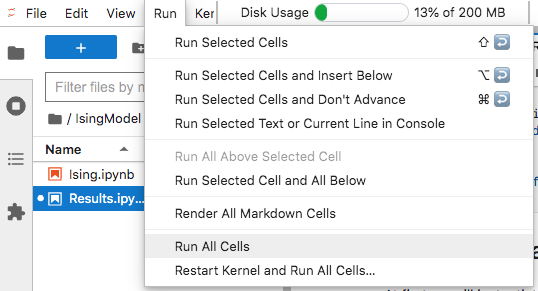
\includegraphics[width=0.75\columnwidth]{img/menu.png}
    \caption{Menu button to execute the whole notebook.}
    \label{fig:menu}
\end{figure}

Alternatively the notebook can be executed cell by cell selecting the cell and pressing the key combination $\keys{\ctrl}+\keys{\return}$ in Windows or $\keys{\cmd}+\keys{\return}$ in Mac.

\subsection{Output}
As outputs of the program we obtain a matrix of $+1$ and $-1$ for the states of the lattice, and for the plots of the observables we had a list of values corresponding with the expected value at a particular temperature. The data then was used to generate images that helped us visualize that data.

\section{Results and Discussion}
Once the model was correctly implemented we were able to generate a lattice and visualize how the model evolves after certain number of Monte Carlo steps (Figure \ref{fig:states}), this step was crucial to understand how the model behaves and be sure that the implementation was faithful to the physical reality.

\begin{figure}[hbt]
    \centering
    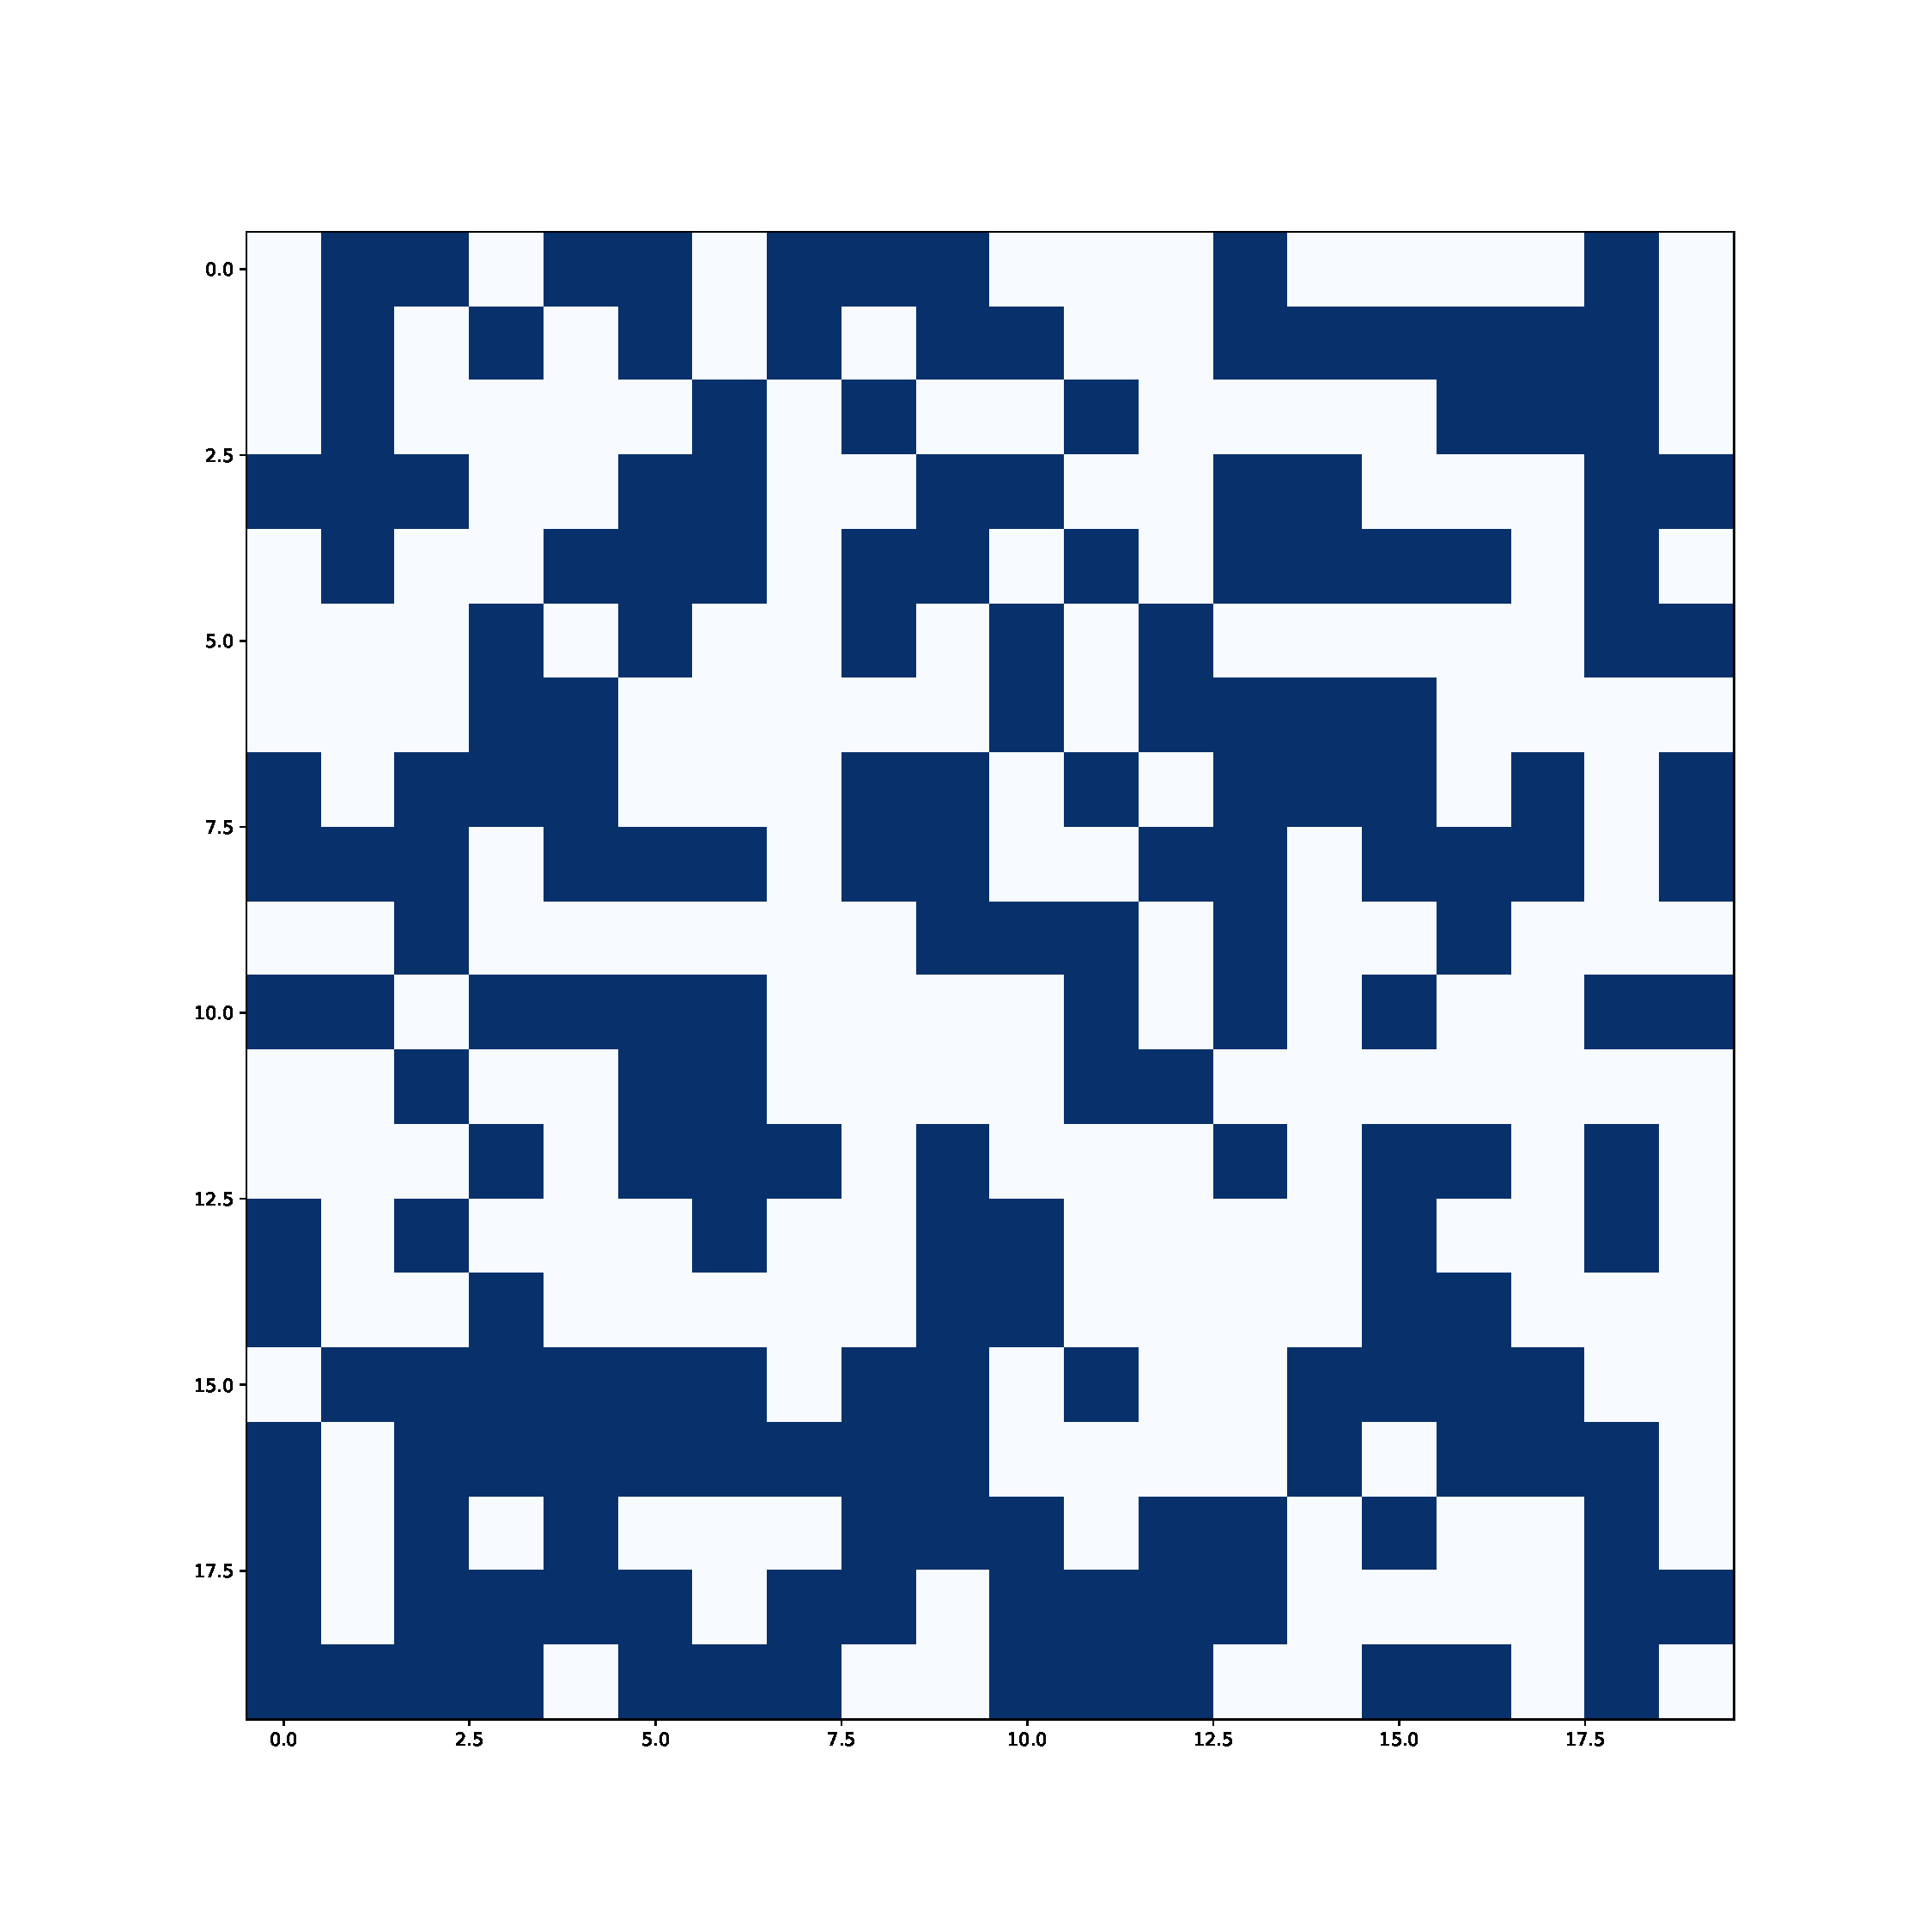
\includegraphics[width=0.49\columnwidth]{img/s0.pdf}
    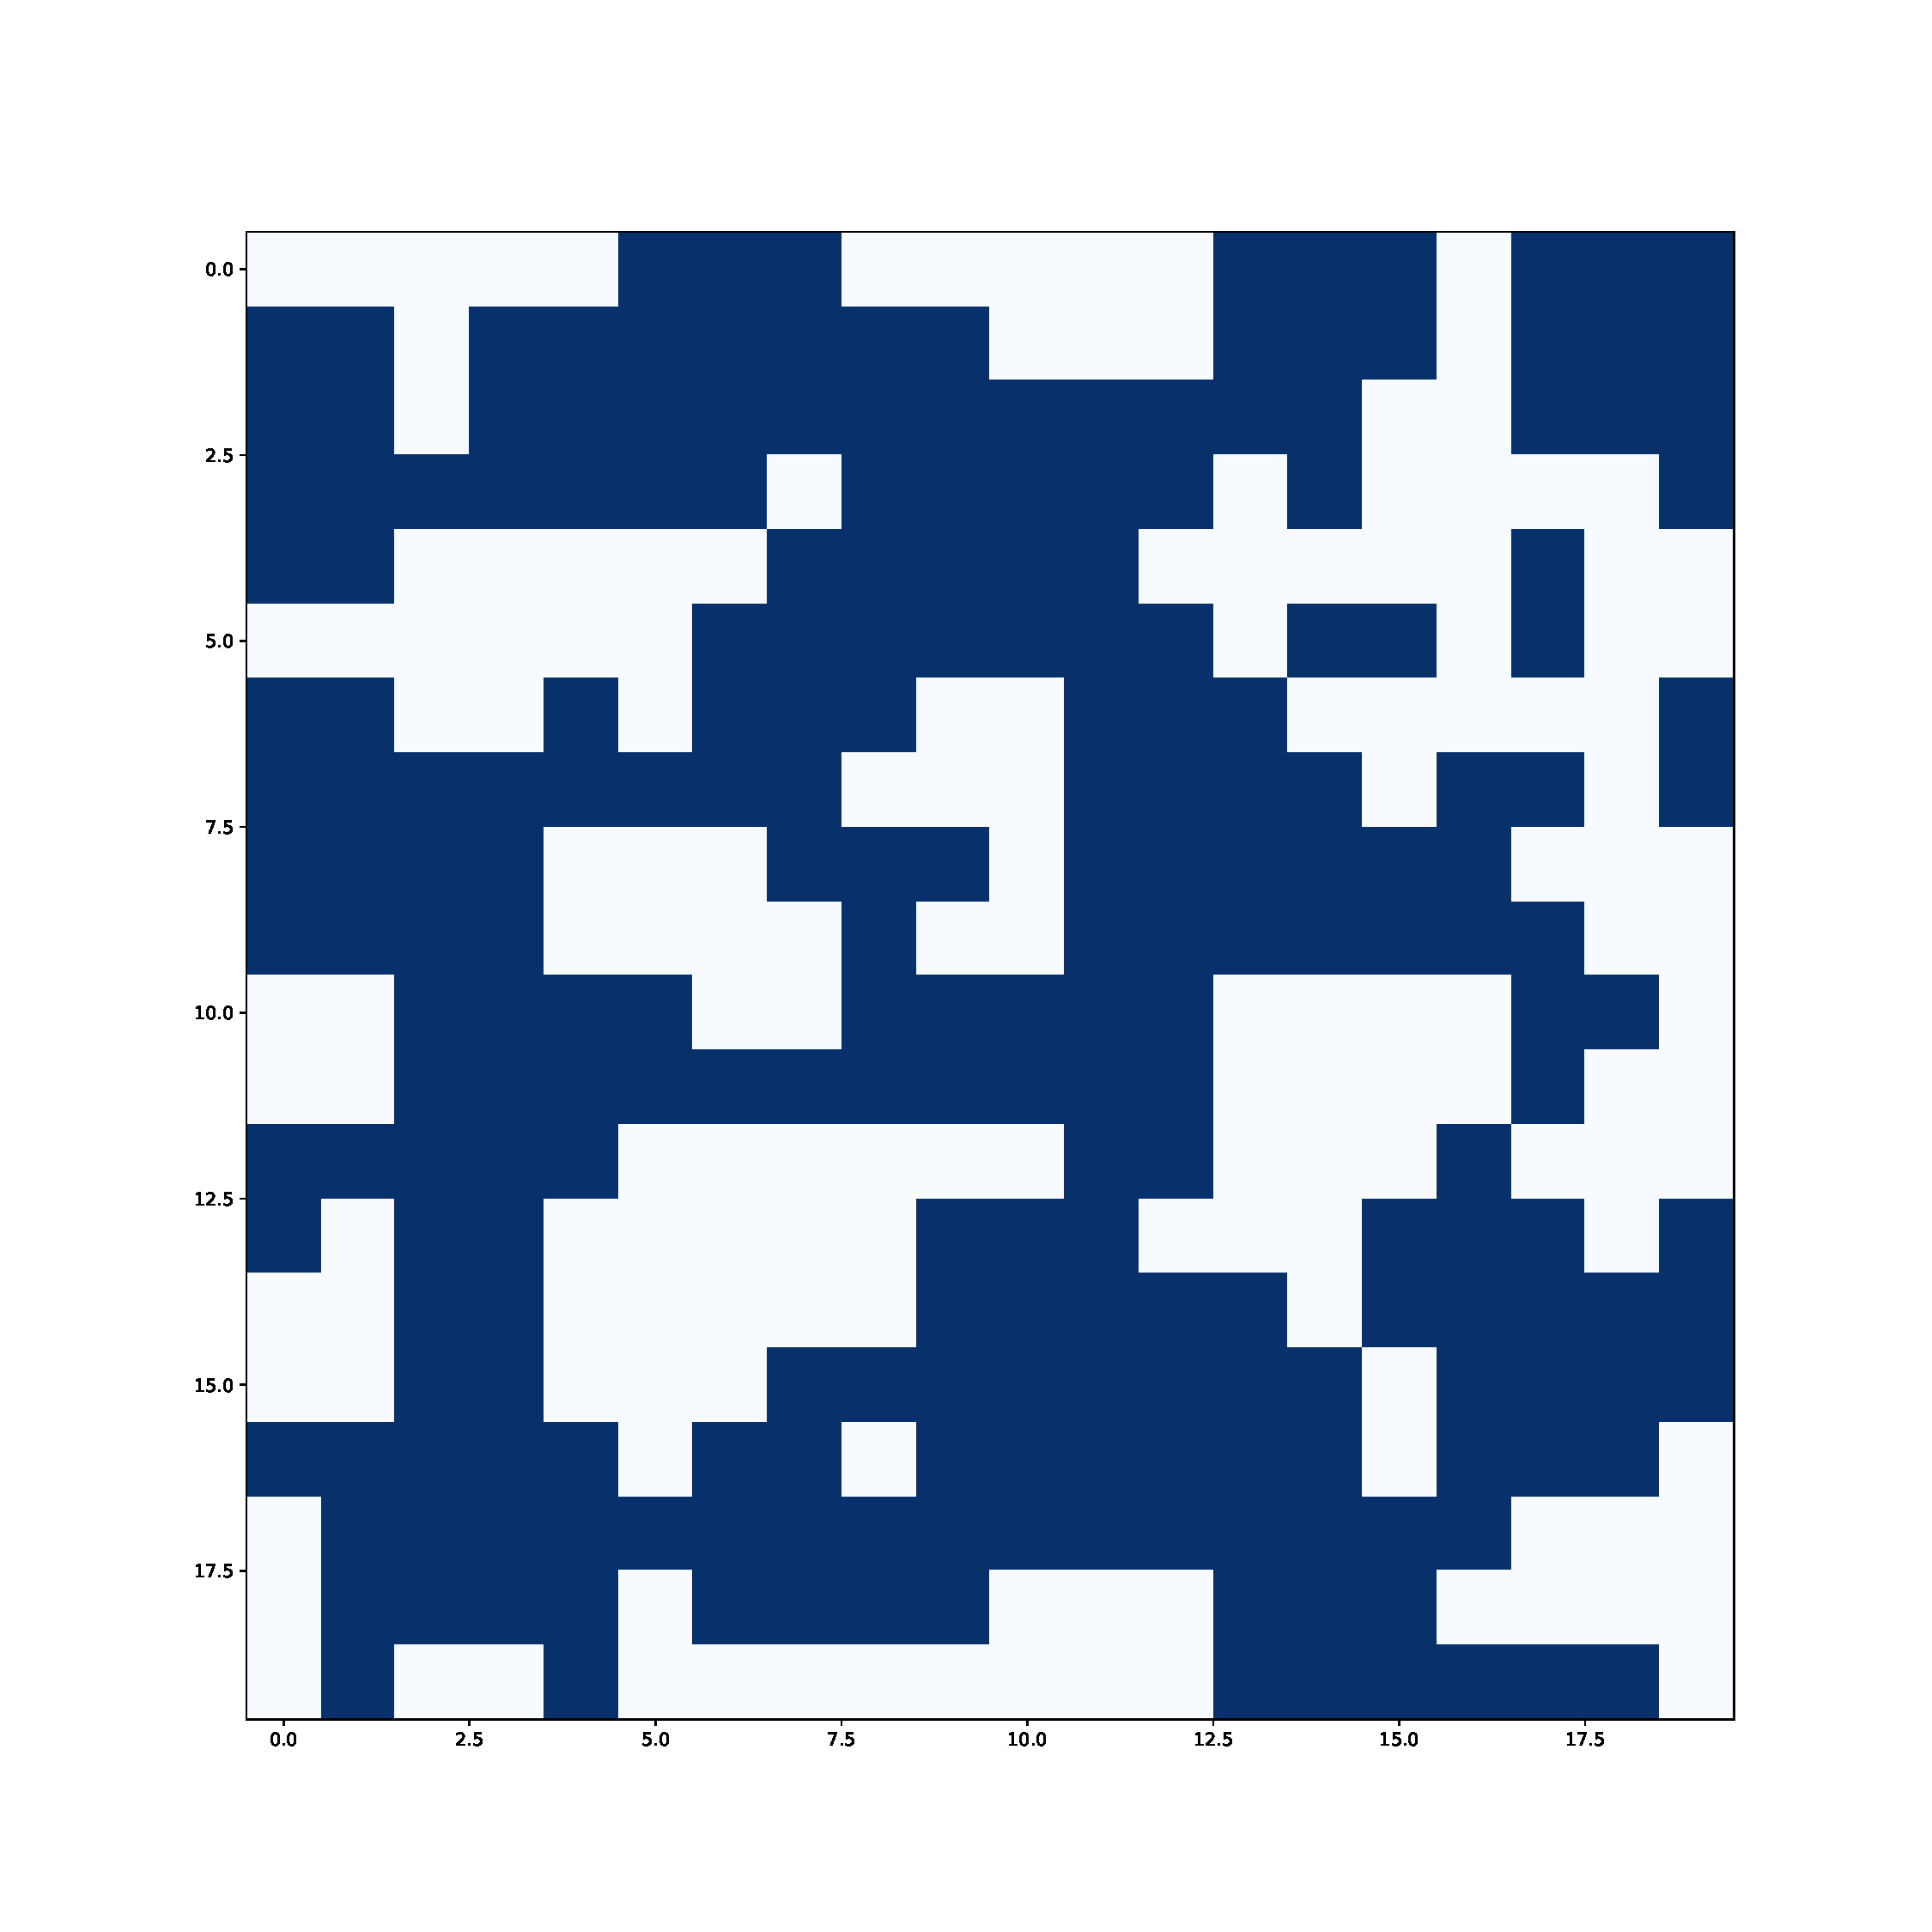
\includegraphics[width=0.49\columnwidth]{img/sf.pdf}
    \caption{Evolution of a $20\times20$ lattice after 500 Montecarlo steps.}
    \label{fig:states}
\end{figure}

We can see in Figure \ref{fig:states} how clusters of magnetization are being generated rather than a noise--alike plot.

Once the model was proven useful for our problem we started the generation of plots for the expected value of energy, specific heat capacity, expected value of magnetization and magnetic susceptibility against temperature. These plots require a big amount of steps to get to an equilibrium state and then to take enough points to obtain a value for the mean that we can trust.

For the energy we where able to accomplish the ``S''--shaped plot that the model should describe as it can be seen in Figure \ref{fig:energy}. Due to the computational limitation it wasn't possible to increase the steps to generate the plots.
\begin{figure}[hbt]
    \centering
    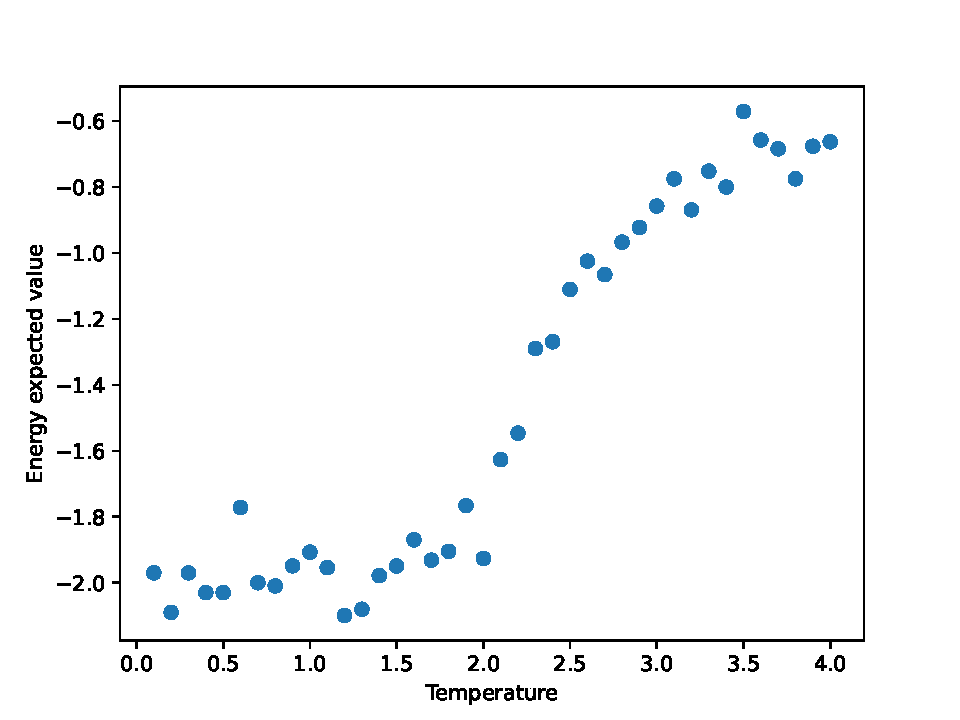
\includegraphics[width=0.95\columnwidth]{img/energy.pdf}
    \caption{$\langle E\rangle$ vs. $T$}
    \label{fig:energy}
\end{figure}

The specific heat capacity was calculated from the energy and is a plot with a very particular shape, since the energy plot was well produced it is not surprising the result obtained in Figure \ref{fig:heat}.
\begin{figure}[hbt]
    \centering
    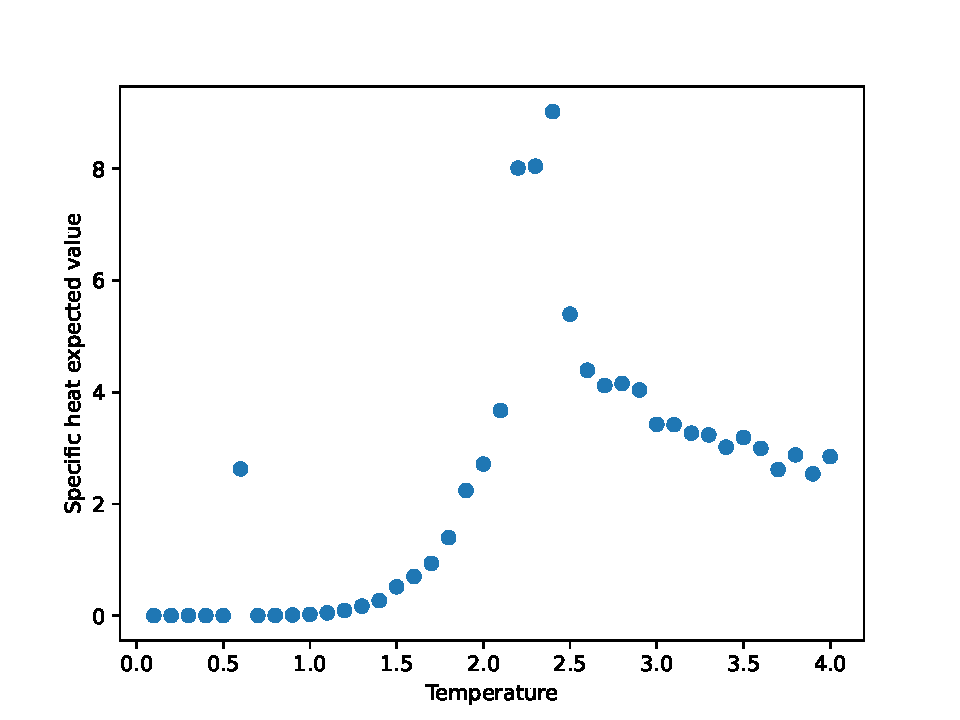
\includegraphics[width=0.95\columnwidth]{img/heat.pdf}
    \caption{$C$ vs. $T$}
    \label{fig:heat}
\end{figure}

In the case of the magnetization we have the bigger differences with other plots. In Figure \ref{fig:magnet} we can see that near to $T=0$ the magnetization value is either $+1$ or $-1$; this happens because of at lower temperatures the material is easily magnetized, but the initial conditions (amount of $-1$ and $+1$ in the initial lattice) is what determines if it is positively or negatively magnetized. And despite of the initial conditions, at bigger temperatures (above the critical temperature) magnetization always tends to 0, as the figure shows. 
\begin{figure}[hbt]
    \centering
    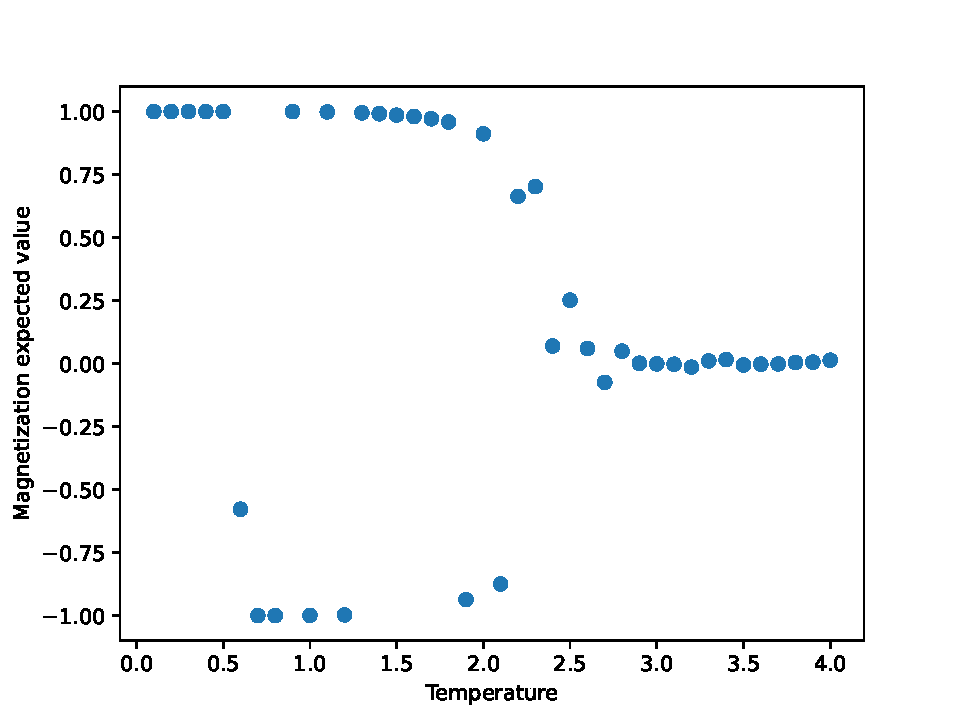
\includegraphics[width=0.95\columnwidth]{img/magnet.pdf}
    \caption{$\langle M\rangle$ vs. $T$}
    \label{fig:magnet}
\end{figure}

Finally, in Figure \ref{fig:chi} we observe a similar shape as in the heat capacity. In this plot the shape is less clear but it is because the width of the spike is lower then the spike in the heat capacity.
\begin{figure}[hbt]
    \centering
    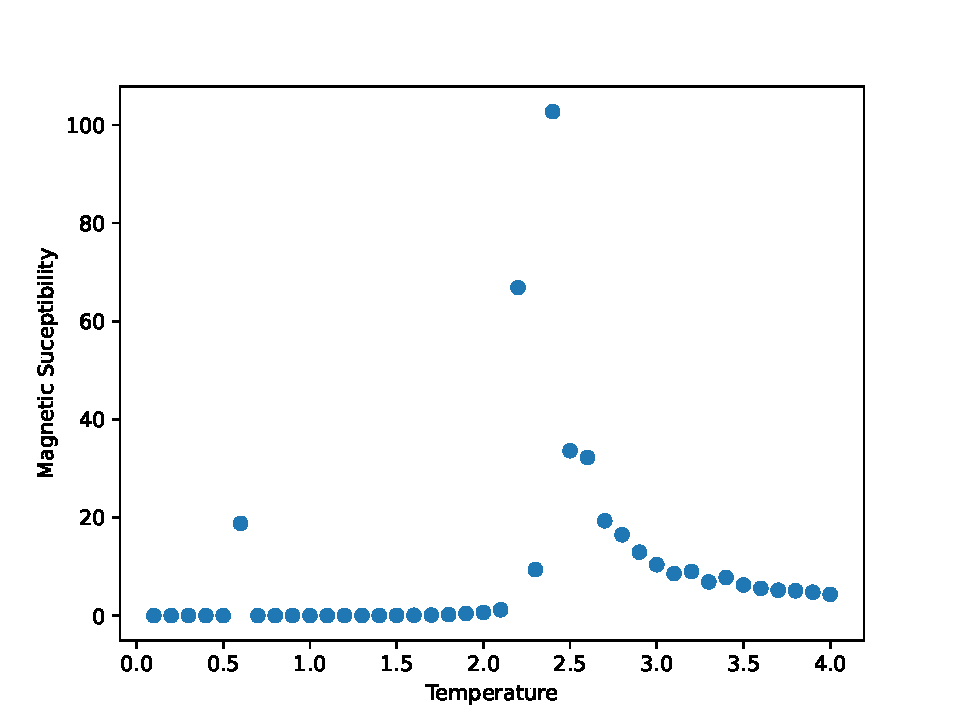
\includegraphics[width=0.95\columnwidth]{img/chi.pdf}
    \caption{$\chi$ vs. $T$}
    \label{fig:chi}
\end{figure}

Additionally, we can see that each plot shows a difference in its behavior when the critical temperature is reached\footnote{Value of critical temperature: $T_c = 2.269185\ldots$, predicted by Onsager \cite{Blundell}.}, showing that the model works as expected.

\section{Conclusion}
We where able to provide a complete implementation of the Ising model based on the class--object paradigm. With that model we could replicate the evolution of a random state through many Monte Carlo steps, and we could also provide plots that illustrate the behavior of different physical properties around the critical temperature point.

\bibliographystyle{IEEEtran}
\bibliography{main}

\appendices

\section{Ising Model Pseudo--code}
This is the pseudo--code abstraction of the model used to later implement the code.
\begin{algorithm}[hbt]
    \centering
    \begin{myalg}[1]
    \LComment{Initialize the lattice of random spins}
    \Require $\Var{m}, \Var{n}, \Var{N}, \Var{T}$
    \Ensure $\Var{m}, \Var{n}, \Var{N} \in \mathds{N}$
    \Ensure $\Var{T} \in \mathds{R}$
    \State $\Var{lattice} \gets \Call{RandomArray}{\Var{m}, \Var{n}}$
    \State $\Var{i} \gets 0$
    \State \null
    \While { $\Var{i} < \Var{N}$ }
        \LComment{Mesure the energy by one spin's sign and the opposite}
        \State $x \gets \Call{URandInt}{0, n}$
        \State $y \gets \Call{URandInt}{0, m}$
        \State $\Var{S} \gets \Call{Take}{\Var{lattice}, x, y}$
        \State $\Var{E}_0 \gets \Call{MesureEnergy}{S, \Var{lattice}, x, y}$
        \State $\Var{E}_1 \gets \Call{MesureEnergy}{-S, \Var{lattice}, x, y}$
        \State \null
        \LComment{Accept state}
        \If{ $\Var{E}_0 > \Var{E}_{1}$ } 
            \State $\Var{S} \gets -S$
        \ElsIf{ $\Call{URand}{0,1} < \exp(-\beta(\Var{E}_1-\Var{E}_0))$ }
            \State $\Var{S} \gets -S$
        \EndIf
        \State $\Var{i} \gets \Var{i} + 1$
    \EndWhile
    \end{myalg}
    \caption{Pseudocode.}
    \label{alg:main}
\end{algorithm}

\section{100 by 100 lattice}
Here are two examples of a $100\times100$ lattice with a difference of a thousand Monte Carlo steps between them, this plots where used to verify the functioning of our model.
\begin{figure}[hbt]
    \centering
    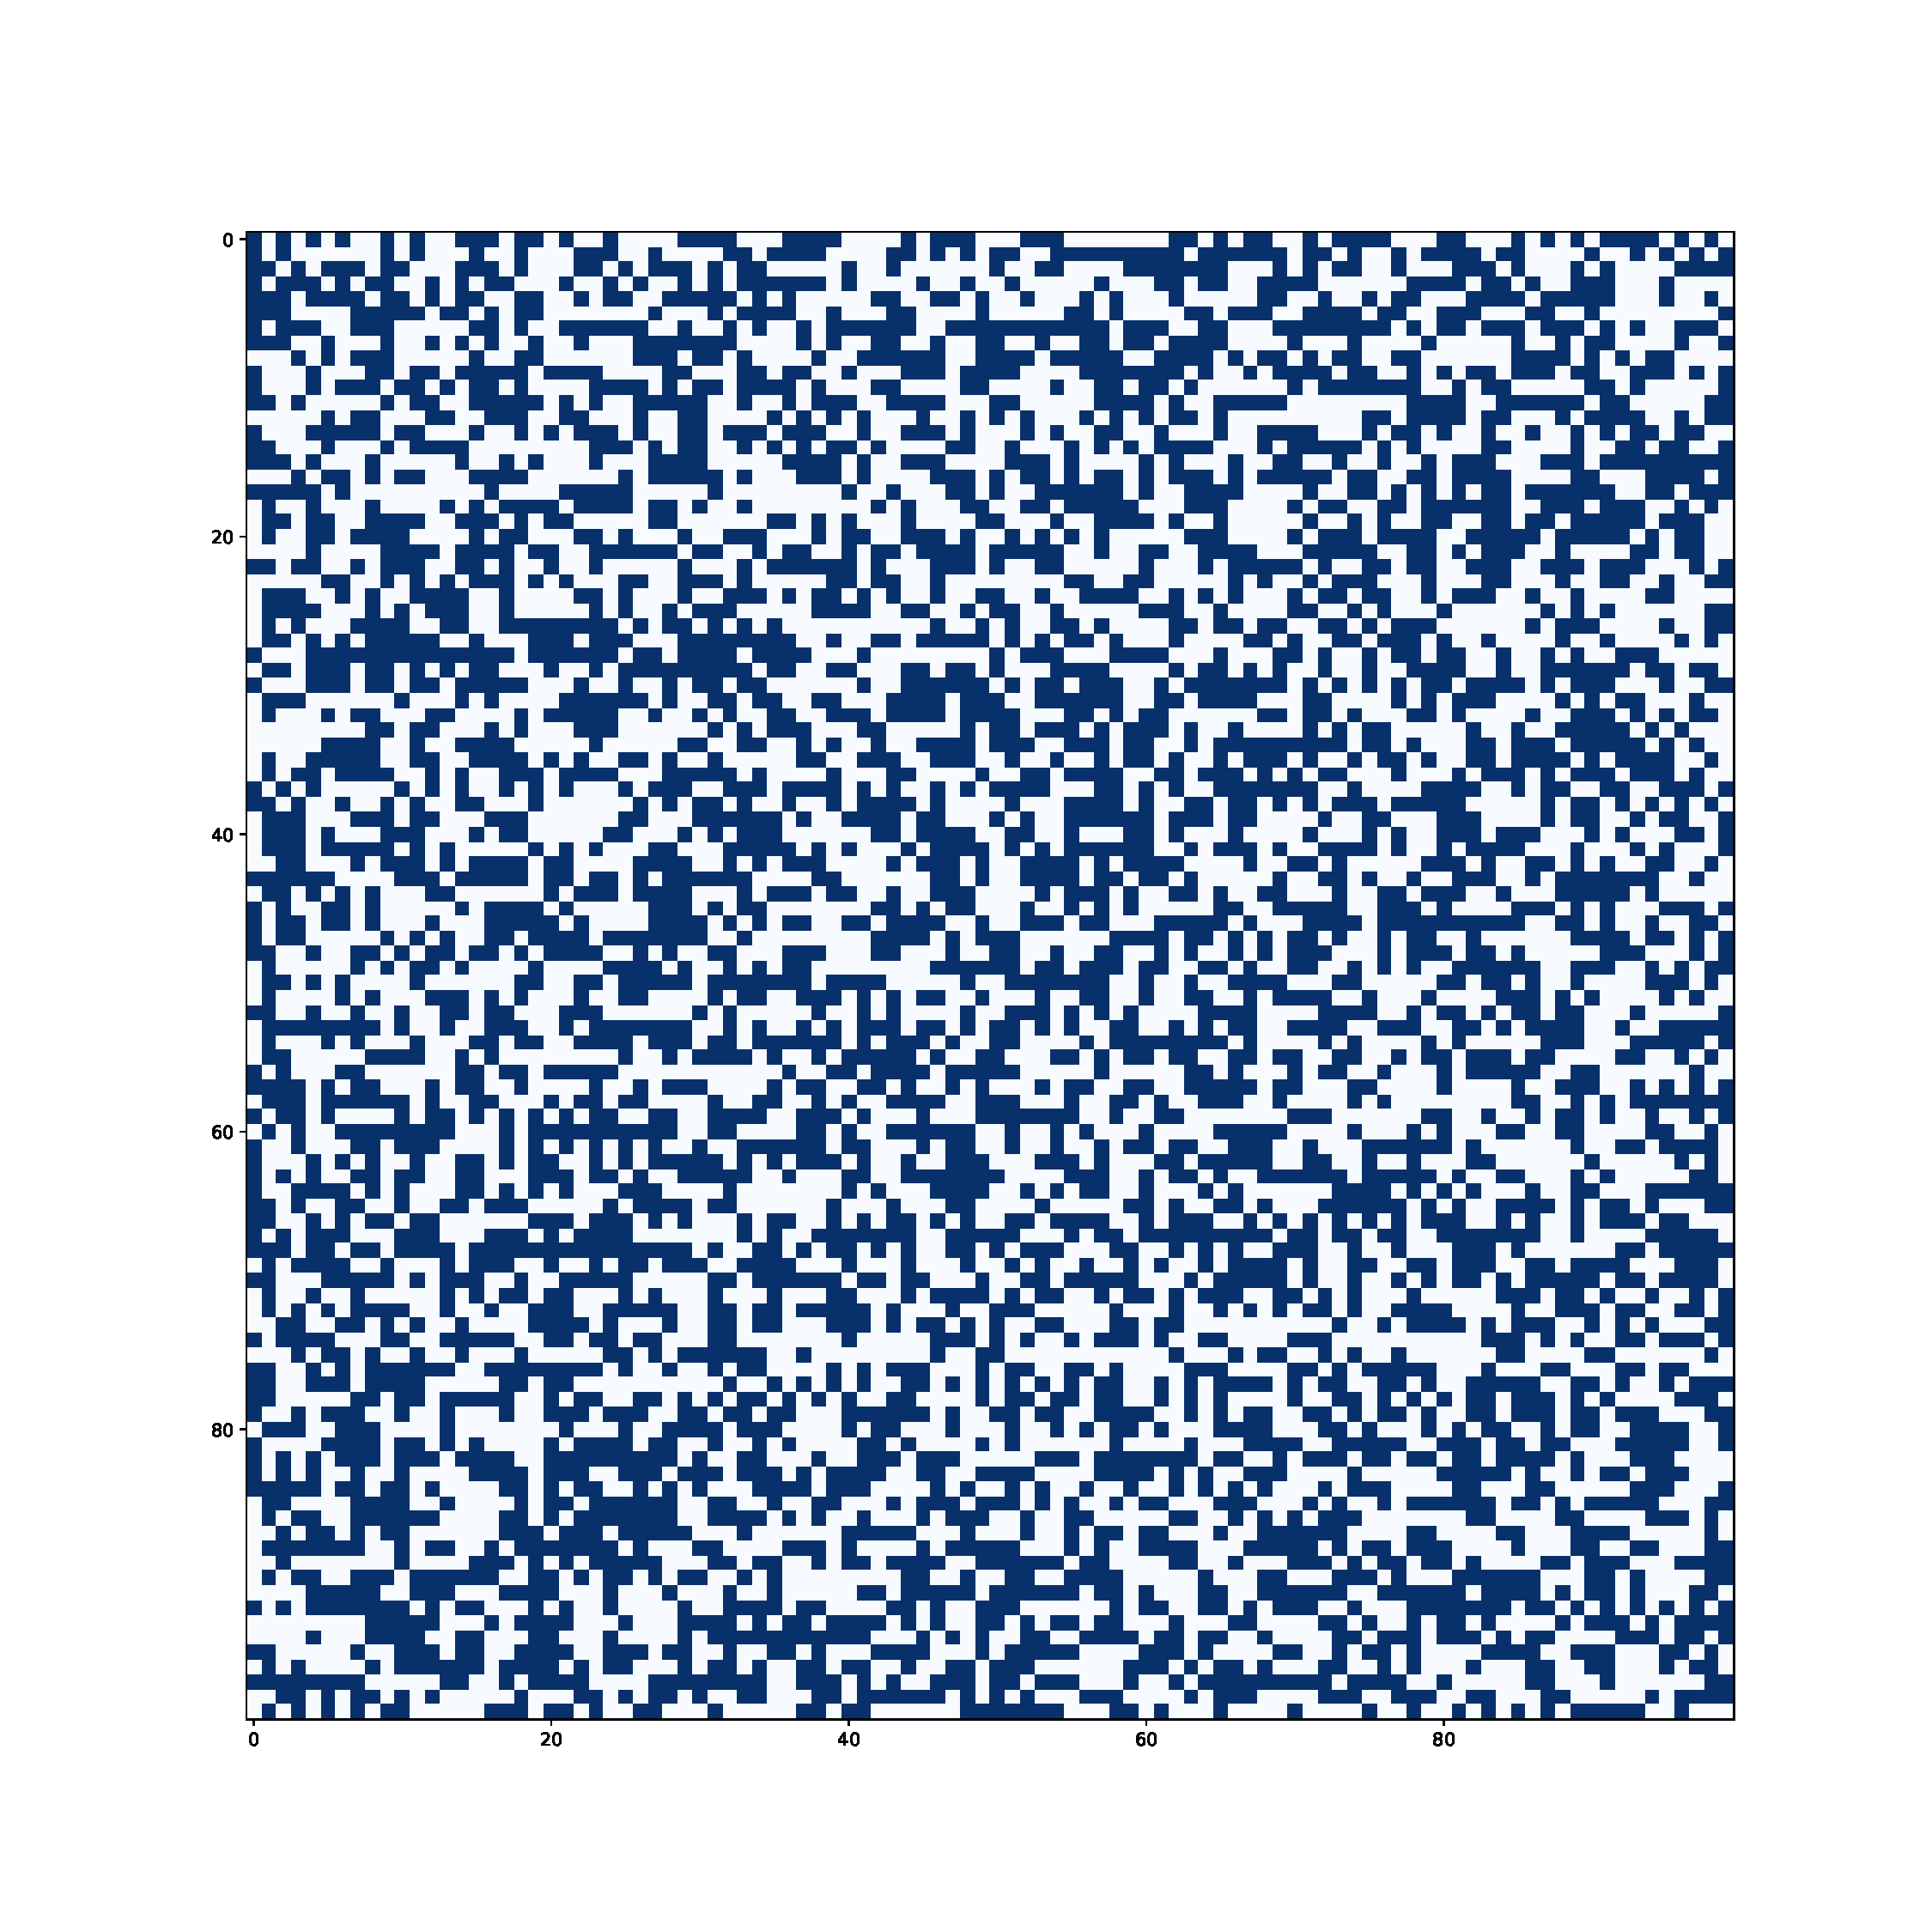
\includegraphics[width=0.7\columnwidth]{img/100i.pdf}
    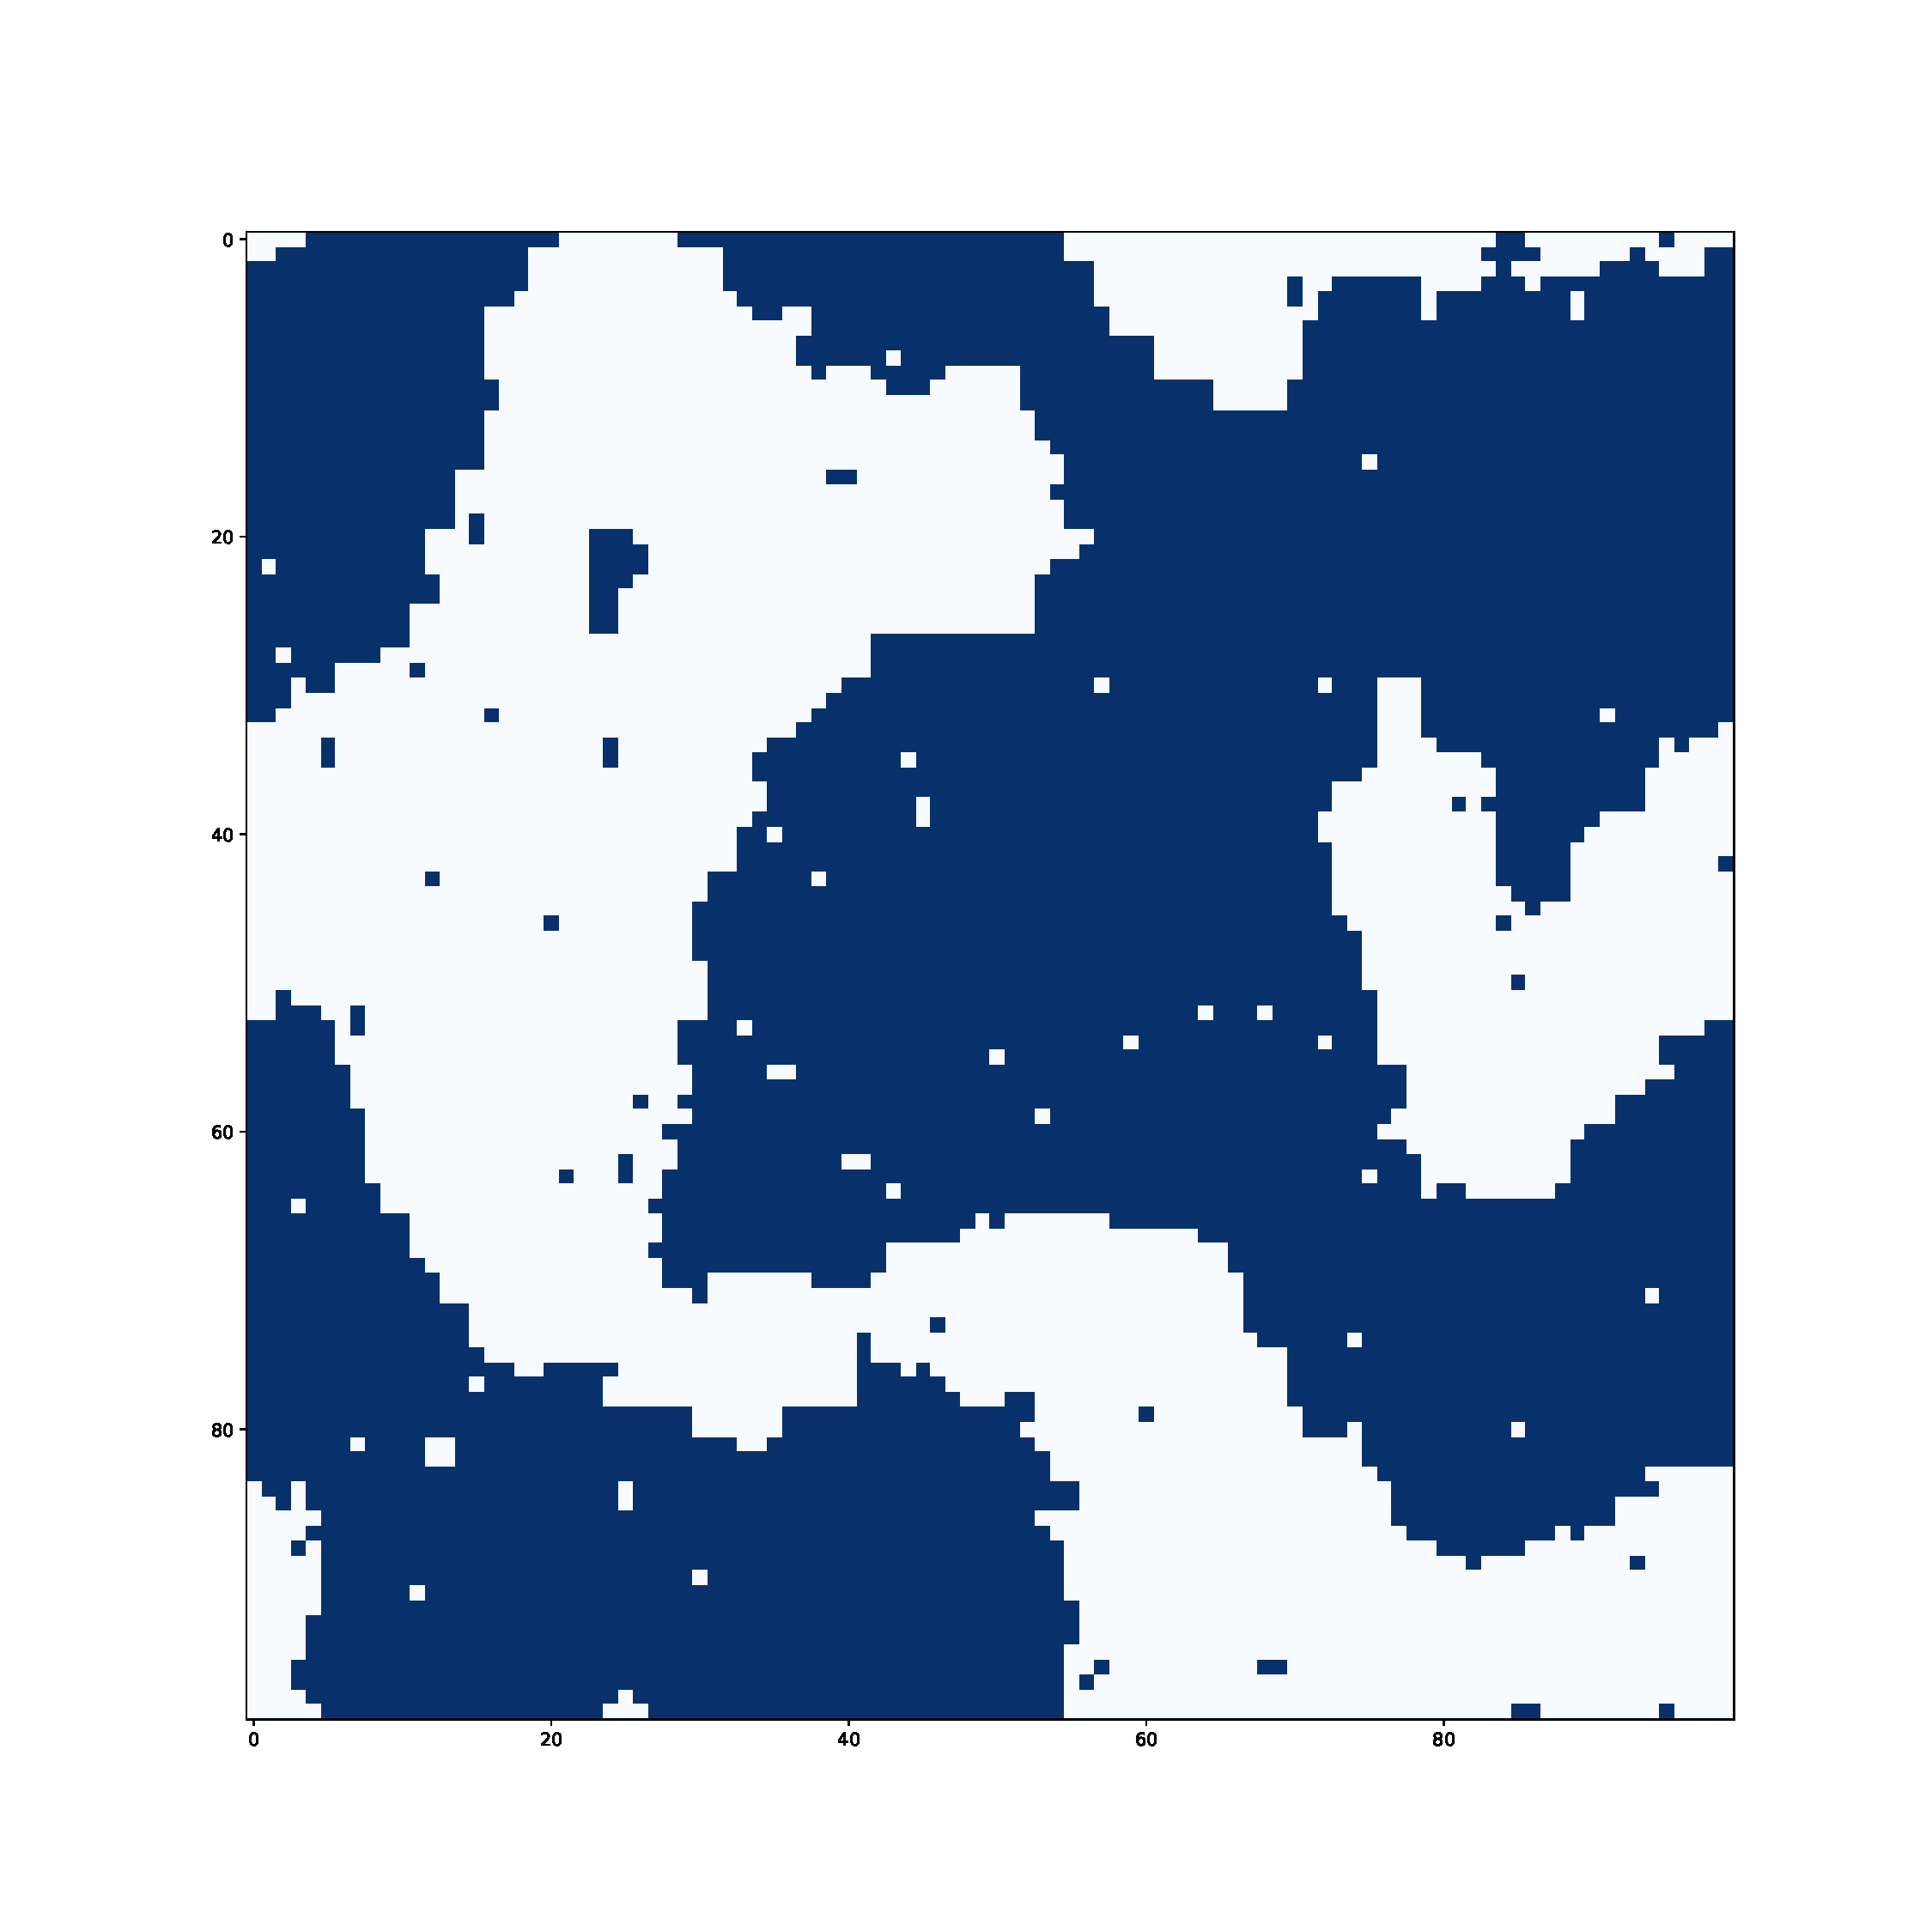
\includegraphics[width=0.7\columnwidth]{img/100f.pdf}
    \caption{$100\times100$ lattice with $1000$ steps.}
    \label{fig:100}
\end{figure}

\end{document}
